\title{Controllo di sistemi lineari}
\maketitle
\label{sec:linear-control}

\paragraph{Introduzione.}

La teoria del controllo applicata ai sistemi lineari è robusta e fornisce tutti gli strumenti necessari
per alterare lo stato di un sistema in modo arbitrario.
In questo capitolo introduco alcuni
concetti di base per studiare il comportamento di un sistema lineare; mostro poi sotto quali
condizioni un sistema lineare è controllabile e infine propongo un criterio per trovare una strategia
ottimale di controllo.

\section{Sistemi lineari}
\subsection{Sistemi dinamici}
Introduco alcuni concetti di base.

\begin{definition}
    Un insieme $\mathcal T \subseteq \R^+$ è detto \textbf{insieme del tempo}.
\end{definition}

\begin{definition}
    Un insieme $\Sigma \subseteq \R^{2n}$ è detto \textbf{spazio delle fasi}
    relativo a un sistema fisico quando i vettori
    $\b x \in \Sigma$ rappresentano tutti gli stati possibili
    del sistema, ovvero,
    tutte le $2n$-uple di coordinate e velocità generalizzate $(q_1, \dot q_1, \ldots, q_n, \dot q_n)$
    possibili per il sistema.
\end{definition}
La richiesta che lo spazio delle fasi abbia dimensione pari è dettata dal
fatto che, in generale, per definire lo stato di un sistema meccanico è
necessario conoscere sia il valore delle coordinate generalizzate
che delle rispettive velocità generalizzate associate.
È possibile definire uno spazio delle fasi che abbia dimensione dispari
oppure che sia un insieme discreto~\cite{Turchetti_1998}, ma ciò non è utile per quanto riguarda
questo testo.

\begin{definition}
\label{def:flusso-di-fase}
    Sia $t \in \mathcal T$ insieme del tempo, $\Sigma$ spazio delle fasi di un sistema e siano $\b x_0, \b x(t) \in \Sigma$.
    L'applicazione: \\
    \begin{equation*}
        \begin{array}{cccc}%
            \phi: &\mathcal T \times \Sigma &\to &\Sigma \\
            &(t, \b x_0) &\mapsto &\b \phi^t(\b x_0) = \b x(t)
        \end{array}%
    \end{equation*}
    è detta \textbf{flusso di fase} se e solo se rispetta le seguenti proprietà:
    \begin{itemize}
        \item \textbf{Identità:} $\phi^0(\b x_0) = \b x_0$.
        \item \textbf{Composizione:} $\phi^t \circ \phi^s = \phi^{t+s}$.
        \raggedright
        \item \textbf{Conservazione della misura:} esiste una misura $\mu$ di $\Sigma$ %
        conservata:
        \begin{equation*}
            \int_A \det J_\phi \ d\mu~=~\int_{\phi^t(A)} d\mu.
        \end{equation*}
    \end{itemize}
\end{definition}

Ora uso le definizioni appena enunciate per introdurre il concetto di
\emph{sistema dinamico}.

\begin{definition}
    La tripla $(\Sigma, \mathcal T, \phi)$ in cui:
    \begin{itemize}
        \item $\Sigma$ è uno spazio delle fasi%
        \item $\mathcal T$ è un insieme del tempo%
        \item $\phi$ è un flusso di fase%
    \end{itemize}
    è detta \textbf{sistema dinamico}.
    \label{def:sistema-dinamico}
\end{definition}

A seconda della scelta di $\mathcal T$, il sistema è detto
\emph{a tempo continuo} oppure \emph{a tempo discreto}.

L'esempio~\ref{ex:semaforo} mostra come è possibile costruire
un semplice sistema dinamico.

\begin{example}
    \label{ex:semaforo}
    Voglio descrivere il comportamento di un semaforo stradale.
    Il semaforo può essere o verde o rosso e cambia colore a intervalli regolari.
    Posso definire lo spazio delle fasi del sistema come:
    \begin{equation*}
        \Sigma = \{\text{Verde}, \text{Rosso} \}.
    \end{equation*}
    Il tempo è discreto: $\mathcal T = \Z^+$ e definisco il flusso di fase $\phi$:
    \begin{equation*}
        \phi^t(\text Rosso) = \left\{
        \begin{array}{lrl}
            Verde &$t$ &dispari\\
            Rosso &$t$ &pari
        \end{array}
        \right.
    \end{equation*}
    \begin{equation*}
        \phi^t(\text Verde) = \left\{
        \begin{array}{lrl}
            Rosso &$t$ &dispari\\
            Verde &$t$ &pari
        \end{array}
        \right.
        .
    \end{equation*}
    La tripla $(\Sigma, \mathcal T, \phi)$ è un \emph{sistema dinamico}.
    Il sistema è illustrato in \autoref{fig:esempio-semaforo}.
    \begin{figure}[H]
        \centering
        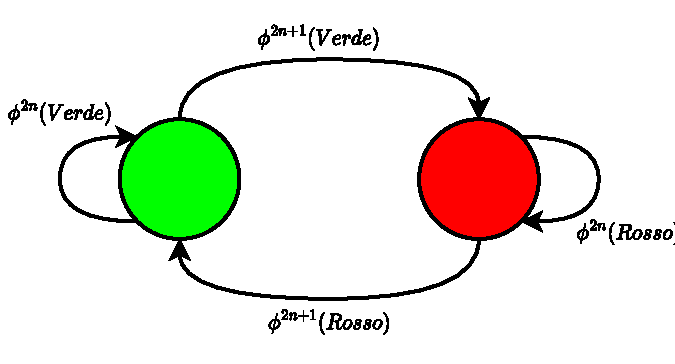
\includegraphics[width=0.5\textwidth]{assets/ex-semaforo}
        \caption[Semaforo]{Esempio di un semaforo come sistema dinamico.
        Gli stati possibili del sistema sono i due colori e il flusso di fase
        regola l'evoluzione temporale del sistema.}
        \label{fig:esempio-semaforo}
    \end{figure}
\end{example}


In generale, dalla osservazione di un sistema fisico si riesce a costruire un campo vettoriale
di equazioni differenziali che ne descrive il moto:
\begin{equation}
    \dot {\b x} (t) = \b a(\b x).
    \label{eq:campo-vett}
\end{equation}
È naturale quindi chiedersi \emph{come e se} sia possibile ricavare il flusso di fase partendo
dal campo vettoriale (e viceversa).
La relazione~\eqref{eq:campo-vettoriale},
analoga alla~\eqref{eq:campo-vett},
mette in relazione ogni sistema di equazioni differenziali con un rispettivo sistema dinamico.
\begin{equation}
    \b a (\b x) = \left.\frac d {dt} \right| _{t=0} \phi^t (\b x_0).
    \label{eq:campo-vettoriale}
\end{equation}

La~\eqref{eq:campo-vettoriale} è, in generale, impossibile da integrare analiticamente.
Per i sistemi lineari, tuttavia, esiste una soluzione in forma chiusa.

\subsection{Equazioni differenziali lineari}
\label{subsec:equazioni-differenziali-lineari}
Introduco la definizione di \emph{equazione differenziale lineare}.
\begin{definition}
    Sia $\b x = \b x(t) \in \R^n$, $A \in \M_{2\times 2}(\R)$, ovvero, lo spazio vettoriale delle
    matrici $n \times n$ a coefficienti reali. Un'equazione nella forma
    \begin{equation}
        \dot{\b x} = A \b x
        \label{eq:sistema-lineare}
    \end{equation}
    è detta \textbf{equazione differenziale} (o sistema di equazioni differenziali) \textbf{lineare omogenea di \rom{1} ordine.}
    \label{def:sistema-lineare}
\end{definition}
\todo {glossario e small caps}

Per le equazioni del tipo~\eqref{eq:sistema-lineare} esiste una soluzione analitica
\begin{equation}
    \b x(t) = e^{\b A t} \b x(0),
    \label{eq:soluzione-lineare}
\end{equation}
dove l'esponenziale di matrice è definito da
\begin{equation*}
    e^{A} = \sum_{k=0}^{+\infty} \frac{A^k}{k!}.
    %\label{eq:exp-matrice}
\end{equation*}

Per dimostrare che la~\eqref{eq:soluzione-lineare} è soluzione, è
sufficiente sostituirla nella~\eqref{eq:sistema-lineare} e verificare che
si ottiene un'identità.
Inoltre, il \autoref{thm:esistenza-unicità} (valido in generale per equazioni
differenziali ordinarie) garantisce che,
fissate le condizioni iniziali, la
soluzione sia unica~\cite{De_Marco_1999}.

\begin{thm}[Esistenza e unicità della soluzione]
    Siano:
    \begin{itemize}
        \item $Y \subseteq \R^n$ spazio di Banach.%
        \item $I \subseteq \R$ intervallo.%
        \item $\b a(t, \b y) : I \times Y \to Y$ continua rispetto a $t$ e lipshitziana rispetto a $\b y$.%
        \item $(t_0, \b y_0) \in I \times Y$.
    \end{itemize}
    Allora il problema di Cauchy
    \begin{equation*}
        \left\{
            \begin{array}{ll}
                \dot{\b y}(t) &= \b a(t, \b y (t)) \\
                \b y (t_0) &= \b y_0
            \end{array}
        \right.
       %\label{eq:cauchy-problem}
    \end{equation*}
    ammette un'unica soluzione $\b \phi$ tale che $\dot {\b \phi}(t) = \b a(t, \b \phi(t))$
    identicamente in $I$ e $\b \phi(t_0) = \b y_0$.
    \label{thm:esistenza-unicità}
\end{thm}

La soluzione~\eqref{eq:soluzione-lineare}
corrisponde al flusso di fase associato al sistema dinamico che ha come campo vettoriale
associato $\b a(\b x) = A\b x$.
Infatti, considerando la proprietà~\eqref{eq:campo-vettoriale} e prendendo
$\phi^t(\b x) = e^{At} \b x$, trovo
\begin{equation*}
        \left. \frac d{dt} \right|_{t=0} e^{At} \b x_0 = A \b x.
\end{equation*}

Questa possibilità di ricavare il flusso di fase partendo dal campo vettoriale per
sistemi lineari è utile, in quanto permette di passare da un sistema a tempo continuo
a un sistema a tempo discreto.
Fissato un intervallo di tempo $\Delta t$, le equazioni~\eqref{eq:mapping-sistema} descrivono lo stesso sistema fisico usando
rispettivamente un insieme del tempo discreto e uno continuo.

\begin{equation}
    \begin{array}{l}
        \mathcal T = \{0, \Delta t, 2\Delta t, \ldots\}, \\
        \b x_{k+1} = e^{A \Delta t} \b x_k
    \end{array}
        \leftrightarrow
    \begin{array}{l}
        \mathcal T = [0, +\infty [, \\
        \dot{\b x} = A \b x,
    \end{array}
    \label{eq:mapping-sistema}
\end{equation}
con $\b x_{k+1} = \b x(k\Delta t)$ e $\b x = \b x(t)$.

Tutte queste considerazioni possono essere estese anche ai sistemi lineari
\emph{non omogenei}.

\begin{definition}
    Sia $\b x = \b x(t) \in \R^n$, $A \in \M_{n\times n}(\R)$, $B \in \M_{n\times m}(\R)$ e $\b u = \b u(t) \in C^0(\R, \R^n)$.
    Un'equazione nella forma
    \begin{equation}
        \dot{\b x} = A \b x + B \b u
        \label{eq:sistema-lineare-non-omogeneo}
    \end{equation}
    è detta \textbf{equazione differenziale} (o sistema di equazioni differenziali) \textbf{lineare non omogenea di \rom{1} ordine.}
    \label{def:sistema-lineare-non-omogeneo}
\end{definition}

La soluzione per equazioni del tipo~\eqref{eq:sistema-lineare-non-omogeneo} è data da
\begin{equation}
    \b x(t) = e^{At} \b x(0) + \int_{0}^{t} e^{A(t-s)} B \b u(s) \ ds.
    \label{eq:soluzione-lineare-non-omogeneo}
\end{equation}
Se si impone che $\b u = \b u_k$ sia costante nell'intervallo di tempo $[k \Delta t, (k + 1)\Delta t]$,
la soluzione prende la forma
\begin{equation*}
    \b x_{k+1} = A_d \b x_k + B_d \b u_k
\end{equation*}
analoga alla~\eqref{eq:mapping-sistema}, con
\begin{equation}
    \begin{aligned}
        A_d &= e^{A\Delta t} \\
        B_d &= \int_0^{\Delta t}e^{As} B\ ds.
    \end{aligned}
    \label{eq:bdequalsint}
\end{equation}
La giustificazione di questa formula è disponibile in~\cite{KAZANTZIS1999763}.

Nel corso di questo testo, userò il termine generale \emph{"sistema"} per indicare
un sistema dinamico a cui è associata un equazione differenziale.
Assumerò che le variabili
coinvolte siano ristrette agli spazi definiti dal sistema dinamico.


\subsection{Linearizzazione di un sistema non lineare}
\label{subsec:linearizzazione}
Considero un sistema dinamico caratterizzato da un campo vettoriale del tipo
\begin{equation}
    \dot {\b x} = \b a(\b x, \b u),\ \text{con}\ \b x = \b x (t)\ \text e \ \b u = \b u (t).
    \label{eq:sistema-non-lineare}
\end{equation}
È possibile linearizzare la dinamica del sistema~\eqref{eq:sistema-non-lineare} in un intorno di un punto fisso
$(\bar{\b x}, \bar{\b u})$ (che, per semplicità, prendo uguale a $(\b 0, \b 0)$) espandendo
in serie di Taylor:
\begin{equation}
    \b a(\b x, \b u) \approx \b a(\b 0, \b 0) +
    \left.\frac{d \b a}{d \b x}\right|_{(\b 0, \b 0)} \b x +
    \left.\frac{d \b a}{d \b u}\right|_{(\b 0, \b 0)} \b u + \mathcal O(\norm{(\b x, \b u)}^2).
    \label{eq:formula-linearizzazione}
\end{equation}
$\b a(\b 0, \b 0)$ si annulla (perché corrisponde a un punto fisso) e posso riscrivere
gli altri due termini in forma matriciale, riconducendomi alla forma~\eqref{def:sistema-lineare-non-omogeneo}
della \autoref{def:sistema-lineare-non-omogeneo}.

Per chiarezza, le matrici $A$ e $B$ sono definite dalla~\eqref{eq:matrici-A-B}.
\begin{equation}
    A_{ij} = \frac{df_i}{dx_j},\ B_{ij} = \frac{df_i}{du_j}.
    \label{eq:matrici-A-B}
\end{equation}
\todo{controlla questa cosa qui perché sono 99\% sicuro che sia giusta ma non ho controllato.}

\subsection{Comportamento asintotico delle soluzioni}
\label{subsec:comportamento-asintotico}
Le soluzioni di un sistema lineare omogeneo possono avere solo uno di tre comportamenti asintotici:
\begin{itemize}
    \item convergere a zero,
    \item divergere,
    \item oscillare attorno a zero.
\end{itemize}
Il comportamento è determinato interamente dagli autovalori della matrice $A$ che definisce il
sistema, secondo la~\eqref{eq:sistema-lineare}.
Le condizioni sufficienti per avere un certo comportamento sono riassunte nella \autoref{prop:comportamento-asintotico}.
\begin{prop}
    Sia $A$ la matrice associata a un sistema di equazioni differenziali omogeneo,
    definita secondo la \autoref{def:sistema-lineare}.
    Se $A$ è diagonalizzabile, il comportamento asintotico delle soluzioni è interamente
    determinato dagli autovalori di $A$:
    \begin{itemize}
        \item Se tutti gli autovalori hanno parte reale \textbf{negativa}, allora $\norm{\b x(t)} \to 0$ per $t \to +\infty$.%
        \item Se almeno un autovalore ha parte reale \textbf{positiva}, allora $\norm{\b x(t)} \to 0$ per $t \to +\infty$.%
        \item Se tutti gli autovalori hanno parte reale \textbf{nulla}, allora le soluzioni sono periodiche.
    \end{itemize}
    \label{prop:comportamento-asintotico}
\end{prop}

\emph{Dimostrazione}.
Lavoro nella base in cui $A$ è diagonale.
In questa base, l'equazione differenziale diventa
\begin{equation}
    \dot{\b z} = \Lambda \b z,
    \label{eq:diagonale}
\end{equation}
dove $\Lambda$ è la matrice che ha sulla diagonale
gli autovalori di $A$ e $\b z, \dot{\b z}$ sono i vettori $\b x, \dot{\b x}$ rappresentati secondo la nuova base.
Sia $T$ la matrice di cambio base, allora $\Lambda$ è data da \todo{la fioresi la chiama così ma dovrei scrivere la definizione...}.
\begin{equation*}
    \Lambda = T^{-1} A T,
\end{equation*}
$\b z$ è dato da
\begin{equation*}
    \b z = T^{-1} \b x
\end{equation*}
e, dato che $A$ non dipende dal tempo, $\dot{\b z}$ è dato da
\begin{equation*}
    \dot{\b z} = T^{-1} \dot{\b x}.
\end{equation*}
Riscrivo la~\eqref{eq:diagonale} in notazione indiciale.
Se $\lambda_i, i = 0, \ldots, n$ sono gli elementi sulla diagonale di $\Lambda$, vale:
\begin{equation*}
    \dot z_i = \delta_{ij} \lambda_i z_j.
\end{equation*}
Mi sono quindi ricondotto a $n$ equazioni differenziali omogenee di \rom{1} ordine, che
hanno come soluzione
\begin{equation*}
    z_i(t) = e^{\lambda_i t},
\end{equation*}
dove ho preso $z_i(0) = 0$.
Gli autovalori sono numeri complessi $\lambda_j = a_j + i b_j$, quindi le soluzioni
sono date dalla~\eqref{eq:soluzioni-complesse}.
\begin{equation}
    e^{\lambda_j t} = e^{a_j t}\left(\cos{b_j t} + i\sin{b_j t} \right).
\label{eq:soluzioni-complesse}
\end{equation}
La dimostrazione termina calcolando il limite per $t \to +\infty$
della~\eqref{eq:soluzioni-complesse} nei tre casi considerati.
\hfill \qedsymbol \paragraph{}

Per i sistemi a tempo discreto le condizioni
sugli autovalori sono fisicamente le stesse,
ma vengono trasformate dalla~\eqref{eq:mapping-sistema} secondo la
seguente proposizione.
\begin{prop}
    Sia $A_d = e^{A\Delta t}$ la matrice associata a un sistema di equazioni differenziali omogeneo
    a tempo discreto:
    \begin{equation*}
        \b x_{k+1} = A_d \b x_k.
    \end{equation*}
    Se $A_d$ è diagonalizzabile, il comportamento asintotico delle soluzioni è interamente
    determinato dagli autovalori di $A_d$:
    \begin{itemize}
        \item Se tutti gli autovalori hanno modulo \textbf{minore di $1$}, allora $\norm{\b x_k} \to 0$ per $k \to +\infty$.%
        \item Se almeno un autovalore ha modulo \textbf{maggiore di $1$}, allora $\norm{\b x_k} \to 0$ per $k \to +\infty$.%
        \item Se tutti gli autovalori hanno \textbf{modulo uguale a $1$}, allora le soluzioni sono periodiche.
    \end{itemize}
\end{prop}
\input{sections/2/controllabilità}
\section{Controllo ottimale: il Regolatore Lineare Quadratico}
\label{sec:controllo-ottimale}
\subsection{Problema di controllo ottimale}
\begin{definition}
    Un problema di controllo per cui è definita una funzione costo
    \begin{equation*}
        J(t) = \phi(\b x) + \int_{\mathcal T} l(\b x, \omega) \ dt
    \end{equation*}
    dove $\phi : \Sigma \to \R$ è una funzione che misura il costo dello stato finale
    e $l : \Sigma \times \mathcal U \to \R$ è una funzione che rappresenta il costo
    della deviazione dallo stato finale per ogni istante di tempo
    è detto \textbf{problema di controllo ottimale}.
\end{definition}
Risolvere un problema di controllo ottimale equivale a ricavare una strategia
di controllo $\omega$ che ne minimizzi la funzione costo.

\subsection{Regolatore lineare quadratico}
Considero un sistema lineare nella forma~\eqref{eq:sistema-lineare-non-omogeneo} controllabile.
Posso formulare un problema di controllo ottimale definendo una funzione costo.
\begin{definition}
    Sia dato un problema di controllo lineare nella forma~\eqref{eq:sistema-lineare-non-omogeneo}.
    Siano $Q \in \M_{n\times n}(\R)$ una matrice semidefinita positiva, $R \in \M_{m\times m}(\R)$ una matrice definita positiva
    e sia definita la funzione costo
    \begin{equation}
        J(t) = \int_0^t
            \left( \b x^{\T} Q \b x + \b u^\T R \b u \right)
        \ ds.
        \label{eq:lqr-cost}
    \end{equation}
    con $\b x = \b x(s)$ e $\b u = \b u(s)$.
    La strategia di controllo $\b u = K\b x$ con $K \in \M_{n\times m}(\R)$ scelta in modo da
    minimizzare la funzione costo~\eqref{eq:lqr-cost} per $t \to +\infty$ è
    detta \textbf{regolatore lineare quadratico (\mysc{LQR}}).
    \label{def:lqr}
\end{definition}
Le matrici $Q$ ed $R$ nella Definizione~\ref{def:lqr} rappresentano rispettivamenge
il costo della deviazione dello stato del sistema da $\b 0$ e il costo dell'attuazione del
controllo.
Nel paragrafo~\ref{subsec:derivazione-riccati} mostrerò che la soluzione per $K$ è
\begin{equation}
    K = R^{-1}BP
    \label{eq:riccati-K}
\end{equation}
dove $P$ è la soluzione all'equazione di Riccati\footnote{Con \emph{equazione di Riccati} ci
si riferisce, in generale, ad un equazione differenziale ordinaria al primo ordine, quadratica nella funzione incognita.}\footnotemark
\begin{equation}
        A^{\T} P + P A - P B R^{-1} B^{\T} P + Q = \b 0.
    \label{eq:riccati}
\end{equation}
La soluzione della~\eqref{eq:riccati} si può trovare numericamente in tempo polinomiale
in $n$~\cite{riccatiO3}.
Nel corso di questo testo, userò la funzione \verb|RiccatiSolve| del software
\emph{Mathematica}~\cite{Mathematica} per risolvere la~\eqref{eq:riccati}.

\footnotetext{Jacopo Francesco Riccati (1676 – 1754) era un matematico
e un giurista. È conosciuto per aver studiato l'equazione che porta il suo
nome.}

\subsection{Derivazione dell'equazione di Riccati}

\label{subsec:derivazione-riccati}
Devo minimizzare la~\eqref{eq:lqr-cost} lungo le traiettorie del sistema.
Uso il metodo dei moltiplicatori di Lagrange e impongo che la variazione totale sia nulla.
\begin{equation*}
    \delta J(t) = \delta \int_0^t
    \left[ \b x^{\T} Q \b x + \b u^\T R \b u  - \b \lambda(\dot{ \b x} - A \b x - B\b u)
    \right]\ ds = \b 0.
    \label{eq:variation-is-zero}
\end{equation*}
La funzione integranda nella~\eqref{eq:variation-is-zero} deve
soddisfare le equazioni di Eulero-Lagrange\footnotemark.
\footnotetext{
    Leonhard Euler (1707 – 1783) è stato un matematico, fisico e astronomo svizzero.
    È considerato il più importante matematico del Settecento, e uno dei massimi della storia. Ha fornito contributi storicamente cruciali in svariate aree: analisi infinitesimale, funzioni speciali, meccanica razionale, meccanica celeste, teoria dei numeri e teoria dei grafi.

    Giuseppe Luigi Lagrangia, naturalizzato in seguito Joseph-Louis Lagrange
    (1736 – 1813), è stato un matematico e astronomo italiano naturalizzato francese.
    La sua più importante opera è la \emph{Mécanique analytique}, pubblicata nel 1788, con cui nasce convenzionalmente la meccanica razionale e analitica.
}
Per chiarezza la indico con $f$ e la riscrivo in notazione indiciale,
in cui sottointendo la somma sugli indici ripetuti.
\begin{equation*}
    f = x_i Q_{ij} x_j + u_l R_{lk} u_k - \lambda_i(\dot x_i - A_{ij} x_j - B_{ik} u_k).
\end{equation*}
Le equazioni di Eulero-Lagrange sono
\begin{equation*}
    \left\{
    \begin{aligned}
        \totald t \partiald{\dot x_a} f - \partiald{x_a} f &= 0, \text{ con } a = 0, \ldots, n, \\
        \totald t \partiald{\dot u_b} f - \partiald{u_b} f &= 0, \text{ con } b = 0, \ldots, m, \\
        \totald t \partiald{\dot \lambda_c} f - \partiald{\lambda_c} f &= 0, \text{ con } c = 0, \ldots, n
    \end{aligned}
    \right.
\end{equation*}
e calcolando le derivate ottengo

\begin{subequations}
    \begin{empheq}[left=\empheqlbrace]{align}
        \dot \lambda_a + 2Q_{aj} x_j + \lambda_i A_{ia} &= 0, \text{ con } a = 0, \ldots, n, \label{eq:sistema-variazionale-1} \\
        2R_{bj}u_j - \lambda_i B_{ib} &= 0, \text{ con } b = 0, \ldots, m, \label{eq:sistema-variazionale-2}\\
        \dot x_c - A_{cj}x_j - B_{ci}u_i &= 0, \text{ con } c = 0, \ldots, n. \label{eq:sistema-variazionale-3}
    \end{empheq}
    \label{eq:sistema-variazionale}
\end{subequations}
Per risolvere il sistema~\eqref{eq:sistema-variazionale} faccio un ansatz
\begin{equation}
    \lambda_a = P_{aj}x_j,
    \label{eq:ansatz-lambda}
\end{equation}
inserisco la~\eqref{eq:ansatz-lambda} nella~\eqref{eq:sistema-variazionale-1} e~\eqref{eq:sistema-variazionale-2} e ottengo
\begin{subequations}
    \begin{align}
        \dot P_{ai}x_i + P_{ai} \dot x_i + 2Q_{ai} x_i + \lambda_i A_{ia} &= 0, \label{eq:sistema-variazionale-4} \\
        2R_{bk}u_k - B_{ib} P_{ij}x_j &= 0 \label{eq:sistema-variazionale-5}
    \end{align}
\end{subequations}
 La~\eqref{eq:sistema-variazionale-3} coincide con l'equazione del moto.
La uso per sostituire $\dot x_j$ nella~\eqref{eq:sistema-variazionale-4}
\begin{equation}
    \dot P_{ai}x_i + P_{ai} (A_{ij}x_j + B_{ik}u_k) + 2Q_{ai} x_i + A_{ia}P_{ij}x_j  = 0.
    \label{eq:sistema-variazionale-6}
\end{equation}
Ricavo $u_j$ dalla~\eqref{eq:sistema-variazionale-5}
\begin{align*}
    2R^{-1}_{lb}R_{bk}u_k &= R^{-1}_{lb} B_{ib} P_{ij}x_j  \\
    \delta_{lk} u_k &= \frac 1 2 R^{-1}_{lb} B_{ib} P_{ij}x_j \numberthis \label{eq:riccati-u}
\end{align*}
e lo sostituisco nella~\eqref{eq:sistema-variazionale-6}.
\begin{equation}
    \dot P_{ai}x_i + P_{ai} (A_{ij}x_j + \frac 1 2  B_{ik} R^{-1}_{kb} B_{mb} P_{mj}x_j) + 2Q_{ai} x_i + A_{ia} P_{ij}x_j = 0.
    \label{eq:sistema-variazionale-7}
\end{equation}
Nella~\eqref{eq:sistema-variazionale-7} l'unico indice libero è $a$.
La riscrivo in notazione matriciale
\begin{equation*}
    \dot P \b x + PA \b x + A^\T P\b x +  \frac 1 2 P B R^{-1} B^\T \b x + 2 Q \b x = 0.
\end{equation*}
Raccogliendo $\b x$ e imponendo $\dot P \to 0$ per $t \to +\infty$ si riottiene
la~\eqref{eq:riccati}. I fattori $2$ e $\frac 1 2$ possono essere rimossi
definendo $P = 2P'$ e dividendo tutto per $2$.
Per ottenere la~\eqref{eq:riccati-K} basta riscrivere
la~\eqref{eq:riccati-u} in forma matriciale.

\hfill\qedsymbol
